\documentclass[10pt,a4paper]{article}
\usepackage[utf8]{inputenc}

% \usepackage{ngerman}  % german documents
\usepackage{graphicx}  % import graphics einbinden
\usepackage{listings}  % support source code listing
\usepackage{amsmath}  % math stuff
\usepackage{amssymb} % 
\usepackage{a4wide} % wide pages
\usepackage{fancyhdr} % nice headers
\lstset{basicstyle=\footnotesize,language=Python,numbers=left, numberstyle=\tiny, stepnumber=5,firstnumber=0, numbersep=5pt} % set up listings
\pagestyle{fancy}             % header
\setlength{\parindent}{0pt}   % no indentation

\usepackage[pdfpagemode=None, colorlinks=true,  % url coloring
           linkcolor=blue, urlcolor=blue, citecolor=blue, plainpages=false, 
           pdfpagelabels,unicode]{hyperref}
           
% change enums style: first level (a), (b), (c)           
\renewcommand{\labelenumi}{(\alph{enumi})}
\renewcommand{\labelenumii}{(\arabic{enumii})}

%lecture name
\newcommand{\lecture}{
	Bioinformatics III
}           

%assignment iteration
\newcommand{\assignment}{
	Second Assignment
}

%set up names, matricle number, and email
\newcommand{\authors}{
  \begin{tabular}{rl}
    \href{mailto:s9alfloh@stud.uni-saarland.de}{Alexander Flohr} & (2549738)\\
    \href{mailto:s9ankupi@stud.uni-saarland.de}{Andrea Kupitz} & (2550260)
  \end{tabular}
}

% use to start a new exercise
\newcommand{\exercise}[1]
{
  \stepcounter{subsection}
  \subsection*{Exercise \thesubsection: #1}

}

\begin{document}
\title{\Large \lecture \\ \textbf{\normalsize \assignment}}
\author{\authors}

\setlength \headheight{25pt}
\fancyhead[R]{\begin{tabular}{r}\lecture \\ \assignment \end{tabular}}
\fancyhead[L]{\authors}


\setcounter{section}{2} % modify for later sheets, i.e. 2, 3, ...
%\section{Introduction to Python and some Network Properties} % optional, note that section invocation sets the section counter + 1, so adapt the setcounter command
\maketitle

\exercise{The scale-free network}
\begin{enumerate}
\item Listing \ref{ex1-1} shows source code.
\lstinputlisting[label=ex1-1,caption={Example Listing of source code}] {ScaleFreeNetwork.py}

\item Listing \ref{ex1-2} shows source code.
\lstinputlisting[label=ex1-2,caption={Example Listing of source code}] {Assign2Task1.py}
Both degree distributions, the one for 1000 and 10000 nodes, follow the same distribution. Only the network with more nodes has some nodes with a higher degree than the other network which seems to result from the higher number of nodes. Figure \ref{fig-1} shows the plot.\\
\begin{figure}
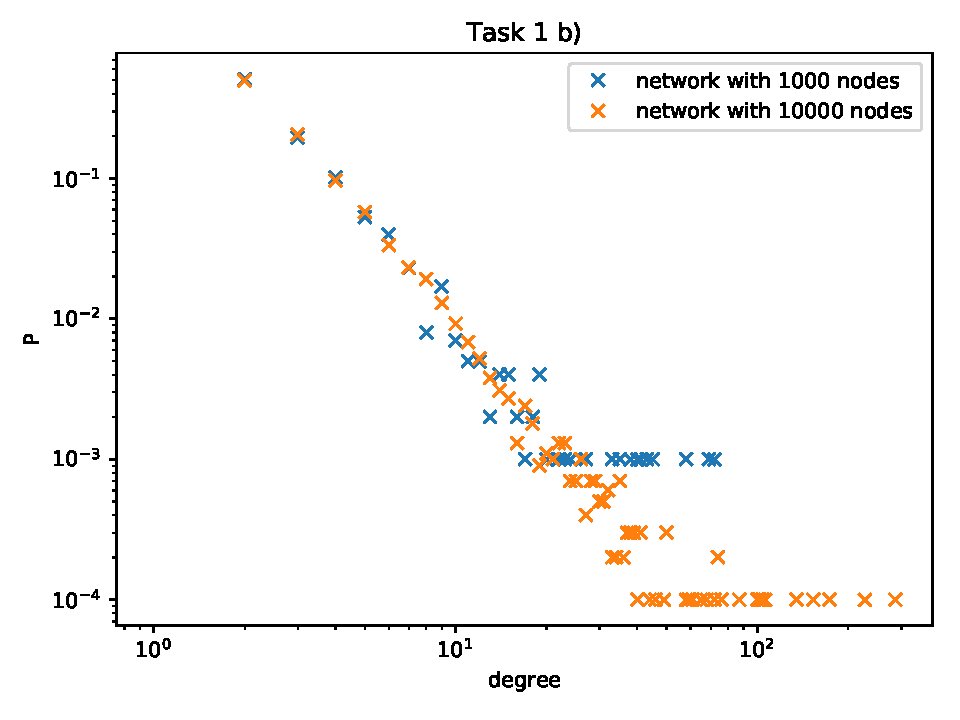
\includegraphics[scale=1]{Figure_1.pdf}
\caption{Comparison of two scale-free networks}
\label{fig-1}
\end{figure}
We also compared a 1000 node scale-free network to a random network of the same size. Unfortunately, because of the higher runtime of the random network generation, we could not finish calculating the corresponding plot.

\item Listing \ref{ex1-3} shows source code.
\lstinputlisting[label=ex1-3,caption={Example Listing of source code}] {Tools.py}
Comparing the empirical and the theoretical distributions, one may see the first third of the graph fit well, whereas the rest of the empirical distribution is very differently distributed. We determined a gamma value of 1.8. The quality of our fit isn't very high. Maybe it could be improved by computing a average distance between each value. Figure \ref{fig-3} shows the plot.
\begin{figure}
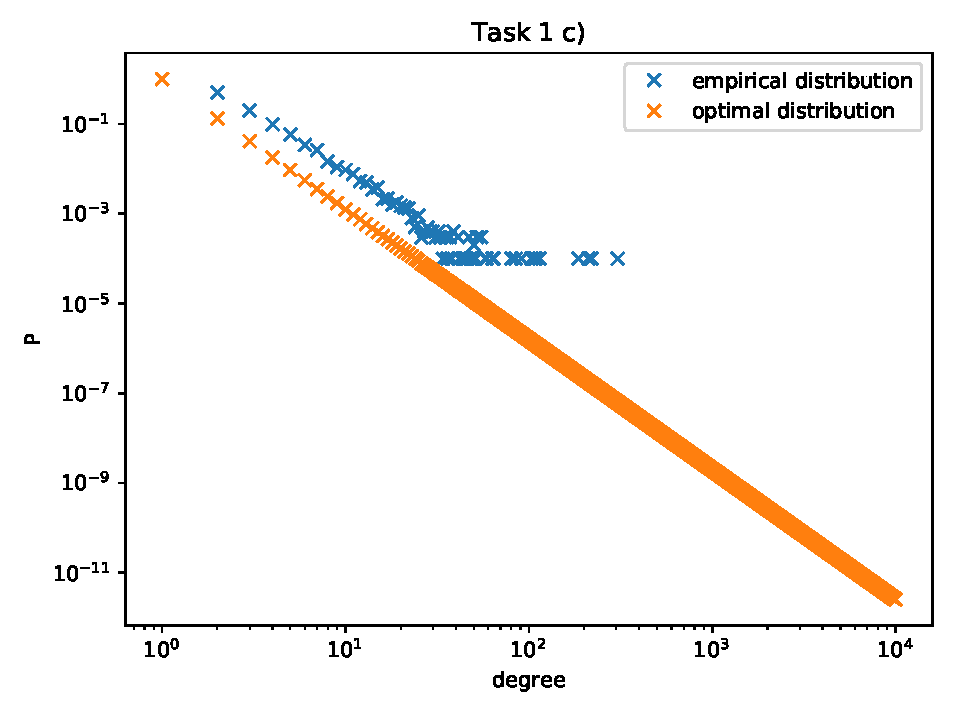
\includegraphics[scale=1]{Figure_3.pdf}
\caption{Comparison of empirical to theoretical network}
\label{fig-3}
\end{figure}
\end{enumerate}

\exercise{Real-world network}
\begin{enumerate}
\item File sharing services like Google Drive form clustered networks, which are clustered by the users which have access to a file. Every time a user adds a new file, a directed link connects a new file to an user.
\item Social networks like Facebook, Twitter and so on may be represented as undirected scale-free networks because people with many friends are more likely to get new friends because they know many people. Moreover a connection between two users is not directed because both users have to accept a friend request.\\
A social network can also be represented as a clustered network, whereby the clustered are made of different groups of friends.
\item Broadcasting networks may form hierarchical or clustered networks. In the case of a hierarchical network, we assume that one broadcaster sends data to multiple other services which publish the data. The network could be clustered by the receiver, which receive data from the same broadcaster. A directed node connects each broadcaster to its receiver.
\end{enumerate}
\newpage
\exercise{Real interaction networks}
\begin{enumerate}
\item Listing \ref{ex2-3-1} shows source code of BioGRIDReader. To retrive all interactions of an organism, use function getInteractions(taxonID)
\lstinputlisting[label=ex2-3-1,caption={Example Listing of source code}] {BioGRIDReader.py}
\newpage
\item Results for organisms with most annotated interactions:
	\begin{table}[!h]
		\caption{List of top five organisms with the most annotated interactions mentioned in the BioGRID}
		\begin{tabular}{|l|l|r|}
			\hline
			Taxon ID & Organism & Number of annotated interaction\\
			\hline\hline
			559292 & \textit{Saccharomyces cerevisiae S288C} & 513254\\
			\hline
			9606 & \textit{Homo sapiens} & 275472\\
			\hline
			316407 & \textit{Escherichia coli str. K-12 substr. W3110} & 181620\\
			\hline
			284812 & \textit{Schizosaccharomyces pombe 972h-} & 58563\\
			\hline
			7227 & \textit{Drosophila melanogaster} & 55093\\
			\hline
		\end{tabular}
		"The genome of Saccharomyces cerevisiae is by far the best studied fungal genome" (\url{https://genome.jgi.doe.gov/Sacce1/Sacce1.home.html}. The human genome is known since the start of the 21th century, and often analyzed since that time. \textit{E. coli} cells are one of the most popular model organisms for laboratory experiments. The same holds true for the fruit fly \textit{Drosophila}. Further, \textit{Schizosaccharomyces pombe 972h-}, or fission yeast is a well known model organism too.\\
		So, beside humans, all top 5 listed organisms are popular laboratory model organisms. Humans are not neccessarily model organisms, but clinical research uncovered many intracellular interaction. Therefore, the list is not surprising.
	\end{table}
\item The human interaction network has 275472 annotated interactions and 17087 nodes.
The top 10 interacting proteins are:

	\begin{table}[!h]
	\caption{Top 10 interacting proteins of humans, annotated in BioGRID, last colum shows evaluation of the Biogrid webpage (\url{https://thebiogrid.org/})}
\begin{tabular}{|l|l|r|c|}
\hline
	ID & Protein & Interactions & reported from BioGrid: Unique Interactor (Interactions)\\
	\hline \hline
	ETG7706			& TRIM25	& 2369 & 2371(2551)\\
	\hline	
	ETG351 			& APP		& 2099 & 2115(2475)\\
	\hline
	ETG4914			& NTRK1		& 1944 & 1943(1999)\\
	\hline
	ETG1994 		& ELAVL1	& 1779 & 1780(1840)\\
	\hline
	ETG7514 		& XPO1		& 1214 & 1236(1315)\\
	\hline
	ETG8452 		& CUL3		& 1209 & 1219(1640)\\
	\hline
	ETG1956 		& EGFR		& 1195 & 1209(2128)\\
	\hline
	ETG10482 		& NXF1 		& 1124 & 1132(1202)\\
	\hline
	ETG7157 		& TP53		& 1011 & 1053(3075)\\
	\hline
	RP11-426L16.2	& MOV10		& 1010 & 1024(1050)\\
	\hline
\end{tabular}
\end{table}	
Hint: The difference in calculated and reported interaction (from BioGRID) can be explained by the fact that our network does not allow multiple links between the same proteins.	Further the differences of unique interaction partners can be partly explained by selfloop wich are ignored in the network.\\
EGFR: This protein is involved in singnaling pathways, which normaly incluedes many protein interactions. Example here is the MAPK cascade in which the protein is involved. Further, EGFR is involved in the transcription of the Polymerase II. Overall, \url{https://thebiogrid.org/} assignes 70 GO annotations to EGFR, 42 for biological processes, 15 for its function and 13 GO components. All these listed annotations hint on activities in which many proteins are involved. This can explain the many interactions, reported in our network.

\newpage	 
\item The function writeInteractionFile is implemented in the class BioGRIDReader, listings \ref{ex2-3-1}. A possible output for human organisms is given in the file human.txt.
Listing \ref{ex2-3-4} shows source code of the generic Network. 
\lstinputlisting[label=ex2-3-4,caption={GenericNetwork class which reads the network from a special file}] {GenericNetwork.py}

The generic network has its own distribution calculation due to an error in the DegreeDistribution class. The degree distribution of our human interaction network can be seen in figure \ref{fig-distribution}. Green colored is the poisson distribution, which we can expect when analyzing a rendom network. It is obvious, that the Human interaction network has a different distribution. The red line, the estimated distribution of a scale-free network on the other hand lokks similar to our distribution. Even if the applied parameters for the red line were not similar to our human distribution.\\
Therefore, the human interaction network behaves more like a scale-free network. 

\begin{figure}
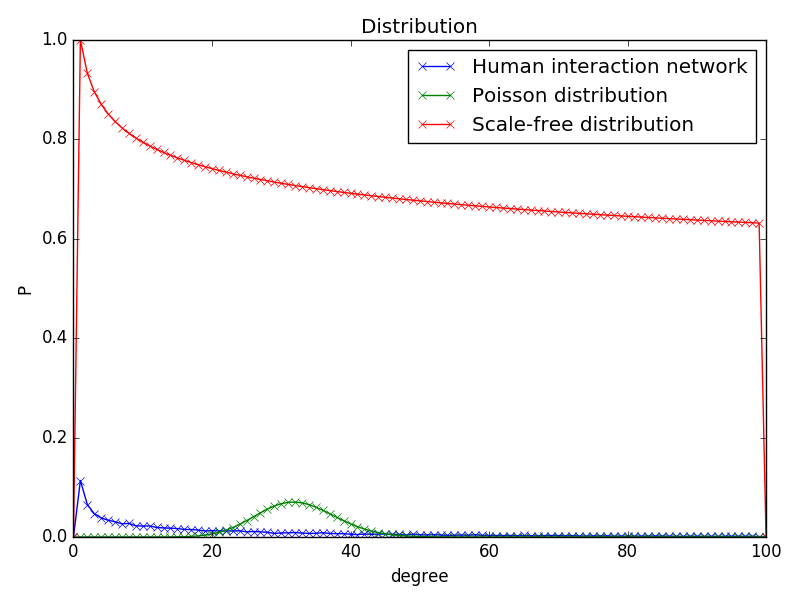
\includegraphics[scale=0.7]{Plot_distribution.png}
\caption{Comparison of empirical to theoretical network}
\label{fig-distribution}
\end{figure}



\end{enumerate}
\end{document}